
\documentclass{bioinfo}
\copyrightyear{2011}
\pubyear{2011}

\usepackage{comment}


\begin{document}
\firstpage{1}

\title{Correcting for bias in high throughput sequencing data}
\author[Jones \textit{et~al}]
{Daniel C. Jones\,$^{1,}$
\footnote{to whom correspondence should be addressed}\hspace{0.5em}
Walter L. Ruzzo\,$^{1,2}$
Xinxia Peng\,$^{3}$
Michael G. Katze$^{3}$
}

\history{Received on XXXXX; revised on XXXXX; accepted on XXXXX}

\address{
$^{1}$Deportment of Computer Science and Engineering, University of
Washington, Seattle, WA 98195-2350, USA\\
$^{2}$Fred Hutchinson Cancer Research Center, Seattle, WA 98109, USA\\
$^{3}$Department of Microbiology, University of Washington, Seattle, WA
98195-7242, USA}

\editor{Associate Editor: XXXXXXX}

\maketitle

\begin{abstract}

\section{Motivation:}
Quantification of sequence abundance in RNA-Seq and ChiP-Seq experiments is
often conflated with protocal-specific bias, influenced by PCR amplification,
and differing primer affinities and mixtures, for example. The result is
potentially inaccurate quantification, affecting de novo gene annotation and
isoform quantification in RNA-Seq, and peak calling in ChiP-Seq.


\section{Results:}
We present a method to measure and correct for these influences using a simple
graphical model. Our model does not rely on existing gene annotations, making it
applicable to any high throughput sequencing data. We evaluate our method on
several datasets, and by multiple criteria, demonstrating that it effectively
decreases bias and increases uniformity.


\section{Availability:}
The method is implemented in the \texttt{seqbias} R/Bioconductor package,
available freely under the LGPL licence from
\href{http://bioconductor.org}{http://bioconductor.org}.


\section{Contact:}
\href{dcjones@cs.washington.edu}{dcjones@cs.washington.edu}

\end{abstract}


\section{Introduction}

In the last few years, RNA-Seq has emerged as a promising alternative to
microarrays in quantifying RNA abundance. But, as microarray technology has
brought with it technical challenges ranging from developing robust
normalization to accounting for cross-hybridization, RNA-Seq presents a new set
of problems.

A significant example is the effect of transcript length on quantification.  As
noted by \citet{Oshlack2009} transcript length biases discovery of
differentially expression, since more reads are aligned to longer transcripts,
granting higher statistical significance in tests differential expression.
Recently, some methods have been developed attempting to account for this effect
in gene set enrichment tests \citep{Young2010,Gao2011}.

%% TODO: do something with this sentance.
Additionally,
differing transcript lengths introduce ``edge effects'', as very short fragments
from the end of a transcript will not be sequenced. NEUMA \cite{Lee2010} and
FPKM \cite{Trapnell2010} are two methods that attempt to take this into account.

The underlying nucleotide sequence also influences quantification in a manner
that is complex and protocol-specific. In an ideal experiment, the number of
reads mapping to a particular position in the genome is a function of RNA
abundance and should not be additionally dependent on the sequence at that
position. As noted first by \citet{Dohm2008}, this is not the case.  As
illustration, Figure \ref{fig:freqs} plots this nonuniformity in nucleotide
frequencies on five data sets (see, Table \ref{tab:datasets}), each using a
different protocol.


These biases may adversely effect transcript discovery, as low level noise may
be over reported in some regions, and in others, active transcription may be
under reported. They render untrustworthy comparisons of relative abundance
between genes or isoforms, and any test of differential expression hangs on the
assumption that these biases are identical between replicates.  Additionally, in
many tests of differential expression---similar to the effects of transcript
length---a higher read count will result in higher statistical confidence. It
follows that the sensitivity of such a test will also be biased by sequence,
affecting downstream analysis such as gene ontology enrichment tests.

This bias, though observed primarily in the 5' end of a read, is not resolved by
trimming the reads prior to mapping \citep{Hansen2010} (see also, Supplementary
Section 1), suggesting it is not a result of erroneous base calling, and that a
more sophisticated means of correction is needed.

\begin{figure*}
\centerline{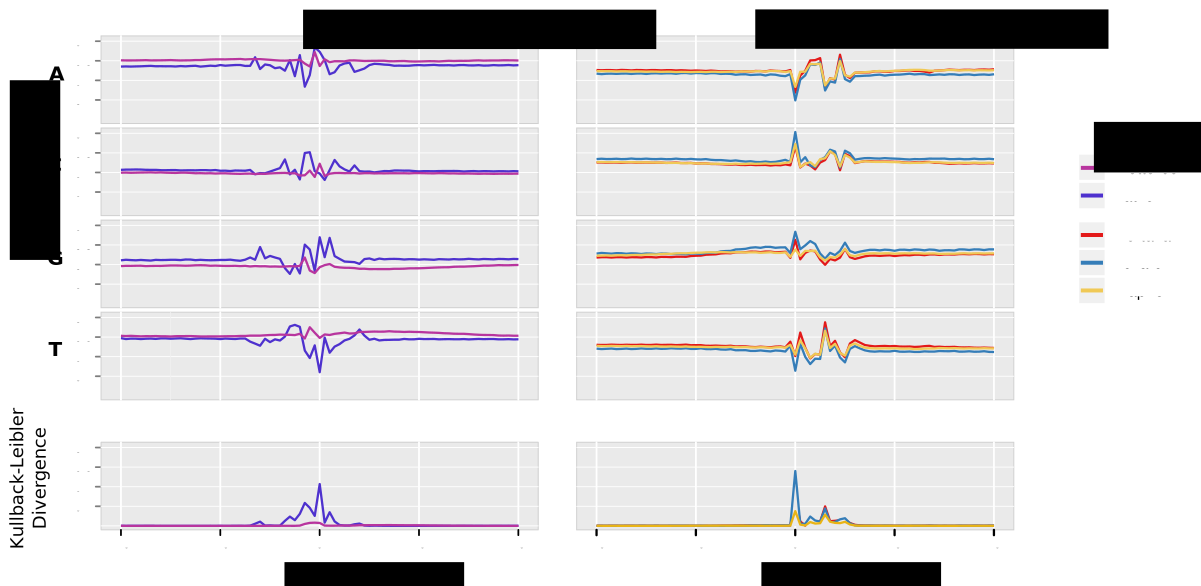
\includegraphics[width=0.8\textwidth]{fig/freqs.eps}}
\caption{Nucleotide frequencies are plotted relative to the start (labeled,
position 0) of each mapped read, respecting strand. The sequence is taken frmo
the genomic context surrounding the read, so that -40 to -1, for example, fall
outside the read sequence itself. The symmetrized Killback-Leibler divergence is
used to summarize the difference in nucleotide frequency compared to a fixed
estimate of background necleotide frequencies made by sampling many positions
nearby mapped reads.  Under the assumption that reads are sampled uniformly from
transcripts, each of the plots should be essentially flat.}
\label{fig:freqs}
\end{figure*}

Li, et. al., \cite{Li2010} propose two models. The first is a Poisson linear
model, in which read counts across a transcript follow inhomogeneous Poisson
process. The read count at position $i$ within the transcript is Poisson
distributed with parameter $\lambda_i$, where, $\log(\lambda_i)$ is the sum of
weights determined by the nucleotide at each position surrounding the read
start, in addition to a term capturing the abundance of the transcript.

The second model is based on multiple additive regression trees, or MART
\citep{Friedman2003}.  In their tests, the MART model shows a moderate
improvement over the Poisson linear model. Both models are fit to a number of
abundant test genes, requiring existing gene annotations for the reference
genome. 

Another model, proposed by \citet{Hansen2010}, directly estimates the
distribution of initial heptamers within reads, then estimates a presumed
background heptamer distribution, sampled from the end of reads. The read count
at a given position is then adjusted by the ratio of the foreground and
background heptamer probabilities. Specifying two distributions over heptamers
(i.e. foreground and background distributions) requires $2(4^7-1) = 32,766$
parameters, so while no gene annotations are needed to train such a model, a
significant number of reads are required.

Lastly, \citet{Roberts2011} have very recently published a description of
another approach, in which sequence probabilities are modeled by variable-order
Markov chains. The structure of these Markov chains are hard-coded, chosen in
advance using a hill-climbing algorithm on a representative dataset. This method
is implemented in the latest version of Cufflinks \citep{Trapnell2010}, and
tightly incorporated into its estimation of transcript abundance.

Here we propose a new approach, using Bayesian networks to model sequence
probabilities. Unlike the methods of Roberts or Li, our model requires no gene
annotations, nor even the assumption that the short reads are derived from RNA.
In this sense, we build on the work done by \citet{Hansen2010}, generalizing
their approach in a way we find to be more robust and effective at correcting
for bias in a variety of protocols. Due to the weak assumptions required my our
model, it is applicable and potentially useful in any setting in which short
reads are aligned to a reference sequence.


%% TODO: where should this figure be cited?
\begin{figure}
\centerline{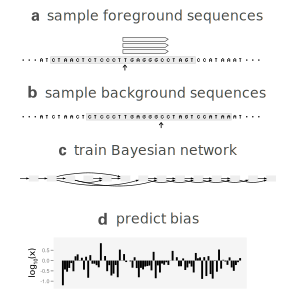
\includegraphics[width=0.35\textwidth]{fig/overview.eps}}
\caption{An overview of the approach taken: (a) foreground sequences are sampled
from the regions surrounding the starts of mapped reads, (b) background
sequences are sampled by randomly offsetting foreground positions, (c) a
Bayesian network is classifier is trained to descriminate between the set of
sampled foreground and background sequences, (d) and the classifier is evaluated
at each position within a locus, predicting bias.}
\label{fig:overview}
\end{figure}

\section{Methods}

\subsection{Principle}

We begin with a natural model of an RNA-Seq experiment (and one that is often
assumed, whether implicitly or otherwise). The number of reads $x_i$ aligned to
genomic position $i$ is an unbiased estimate of RNA abundance. Furthermore, we
assume reads may be treated as independent and identically distributed samples.
That is, if $N$ reads are generated, and $m_i$ is the event that a generated
read maps to position $i$.
$$ E[x_i] = N \Pr[m_i] $$

The experiment may be considered unbiased  with regards to sequence if, having
observed the nucleotide sequence $s_i$ surrounding position $i$,
$$ E[ x_i | s_i ] = N \Pr[ m_i | s_i ] = N \Pr[ m_i ] = E[ x_i ] $$

From Bayes' rule,
$$ \Pr[ m_i | s_i ] = \frac{ \Pr[ s_i | m_i ] \Pr[ m_i ] }{ \Pr[ s_i ] } $$

This suggests a natural scheme in which observations may be reweighted to
correct for bias.  First, define the \emph{sequence bias} $b_i$ at position $i$
as,
$$ b_i = \frac{ \Pr[ s_i ] } { \Pr[ s_i | m_i ] } $$

Now, if we reweight the read count $x_i$ at position $i$ by $b_i$, we
have,
\begin{align*}
E[ b_i x_i | s_i ] &= b_i E[ x_i | s_i ] \\
&= N b_i \Pr[ m_i | s_i ] \\
&= N \frac{ \Pr[ m_i | s_i ] \Pr[ s_i ] }{ \Pr[ s_i | m_i ] } \\
&= N \Pr[ m_i ] \\
&= E[ x_i ]
\end{align*}
Thus the reweighted read counts are made unbiased.

To estimate the bias $b_i$, we must make estimates of the background sequence
probability $\Pr[s_i]$ and the foreground sequence probability $\Pr[ s_i | m_i
]$, the latter being the probability of the sequence given a read being sampled
from its position. Estimating bias is therefore a problem of finding a model of
sequence probability that sufficiently complex to capture the common features of
the training data yet avoids overfitting.

Towards that end, we propose training a Bayesian network classifier trained on
examples of foreground and background sequences. Though our goal is not
classification, by using the machinery of classification we can avoid a model
that is over-parametrized. Parameters that are not informative in
discriminating between foreground and background are not included in the model.
The Bayesian network can then used to evaluate sequence probability, and thus
bias, at any genomic position.

However, we have so for ignored one complication: the RNA abundance that we wish
to estimate is not itself independent of the nucleotide sequence. Notably,
exonic DNA tends to be more GC-rich than intergenic DNA. If background sequences
are sampled uniformly from the genome we run the risk of incorrectly adjusting
for biological sequence bias, rather than techncical sequence bias.  To avoid
this, we propose using paired training data. Each foreground training
sequence is paired with a background sequence taken from nearby position
that is likely to have similar abundance and general nucleotide composition.
Alternatively, we could pair foreground samples with background samples from
within the same transcript, but we prefer to avoid dependence on existing
gene annotations as such a model would be limited to RNA-Seq analysis in which
trustworthy and reasonably complete gene annotations are available.

The methods proposed \citet{Hansen2010} and \cite{Roberts2011} also treat bias
correction as a problem of estimating foreground and background sequence
probabilities. They differ primarily in how these sequence probabilities are
estimated. \citet{Li2010} estimate reweighting coefficients ($b_i$, in our
notation) directly, given training data consistig of long, highly-expressed
transcripts.



\subsection{Estimation}

To estimate sequencing bias, we train a Bayesian network classifier in which
each node represents a position in the sequence, relative to the read start, and
edges encode dependency between positions.  Bayesian networks have been applied
to recognize motifs in nucleotide sequences in the past, in particular in
modeling splice sites \citep{Cai2000, Chen2005} and transcription factor binding
sites \citep{Ben-Gal2005, Grau2006, Pudimat2005}. 

In our model, we do not rely on constraining the set of networks (e.g. to
trees), and instead approximate the NP-Hard problem of determining the optimal
network structure using a fast hill climbing algorithm. Furthermore, we
train our model \emph{discriminatively}; only parameters that are deemed
informative in discriminating between foreground and background sequences are
included in the model. We thus seek to train a model that reduces bias, without
including uninformative parameters that would only increase variance.


\subsubsection{Sampling}

The model is trained on $n$ sequences, one half labeled as foreground, the other
background, sampled from the reference genome. To obtain the foreground
sequences, we take sequences surrounding the starts positions of $n/2$ aligned
reads. We wish to avoid overfitting to any short locus with a large abundance of reads,
yet we must also capture the bias introduced by PCR amplification. We therefore
choose the $n/2$ unique reads with the highest number of duplicates,
yet count each read only once, ignoring duplicates

To obtain background training sequences, we randomly offset the positions from
which the foreground sequences were sampled.  The offset is drawn from a
zero-mean gaussian, and rounded to the nearest integer, away from zero.
By using such a scheme, we attempt to mitigate the effects of biological
sequence bias, sampling positions that are more likely to be biologically
similar.

This procuder produces a training set of $n$ sequences with accompanying labels
$T = \{ (s_1, x_1), (s_2, x_2), \dots, (s_n, x_n) \}$. The label $x_i$ is
binary, indicating classification as background ($x_i = 0$) or foreground ($x_i
= 1$).

\subsubsection{Training}


To determine the structure and parameters of the Bayesian network, we use a
hill-climbing approach similar to algorithm described by \citet{Grossman2004}.
The network structure is determined by greedily optimizing the conditional
log-likelihood.
\begin{align*}
\ell &= \sum_{i=1}^{n} \log \Pr( x_i | s_i ) \\
&=
\sum_{i=1}^{n} \log \frac{ \Pr(s_i | x_i) \Pr( x_i ) }{
\sum_{x \in \{0,1\}} \Pr( s_i | x ) \Pr(x) } \\
\end{align*}

Where $\Pr(x)$ is flat (i.e.  $\Pr( x = 0 ) = \Pr( x = 1 ) =
0.5$) if we sample foreground and background positions equally.

As we will be estimating parameters and evaluating the likelihood on the same
set of samples, simply maximizing the likelihood would severely overfit the
training set. We thus penalize model complexity heuristically using the Akaike
information criterion. Where $m$ is the number of parameters needed to specify
the model, we maximize, 

$$ \ell' = \ell - m $$

Some benifit would be obtained from a more highly tuned complexity penalty.
However, since the model is trained greedily, additional parameters will be
decreasingly informitive, and increasingly similar between foreground and
background. Adding more parameters will have little effect.  Only when $m$ is
allowed to grow exponentially does the prediction become polluted by small
deviations between thousands of uninformitive parameters.

At each step of the optimization procedure, every possible edge or position
addition, removal, or edge reversal that produces a valid network (i.e., does not
introduce a cycle) is evaluated, and the alteration that increases the score
$\ell'$ the most is kept.  This process is repeated until a local maximum is
found, in which no single alteration to the network will increase the score.

Given the network structure, the parameters are estimated directly from the
observed nucleotide frequencies in the training data.

The run time of the training procedure is further reduced in practice by imposing the
following two restrictions on the structure of the network,
\begin{enumerate}
\item The in-degree (i.e. number of parents) of any node must be less than some
number $p_{\text{max}}$.
\item $|j - i| \le d_{\text{max}}$ for all edges $(i,j)$ and some number $d_{\text{max}}$.
\end{enumerate}
The second of these encodes the assumption that distant nucleotides are
effectively independent. We choose $p_{\text{max}} = 4$ and $d_{\text{max}} =
10$, as reasonable default values.

Figure \ref{fig:models} shows examples of the structure learned when this
procedure is applied to several data sets, using 200,000 reads from each.


\section{Results}

\begin{figure*}
\centerline{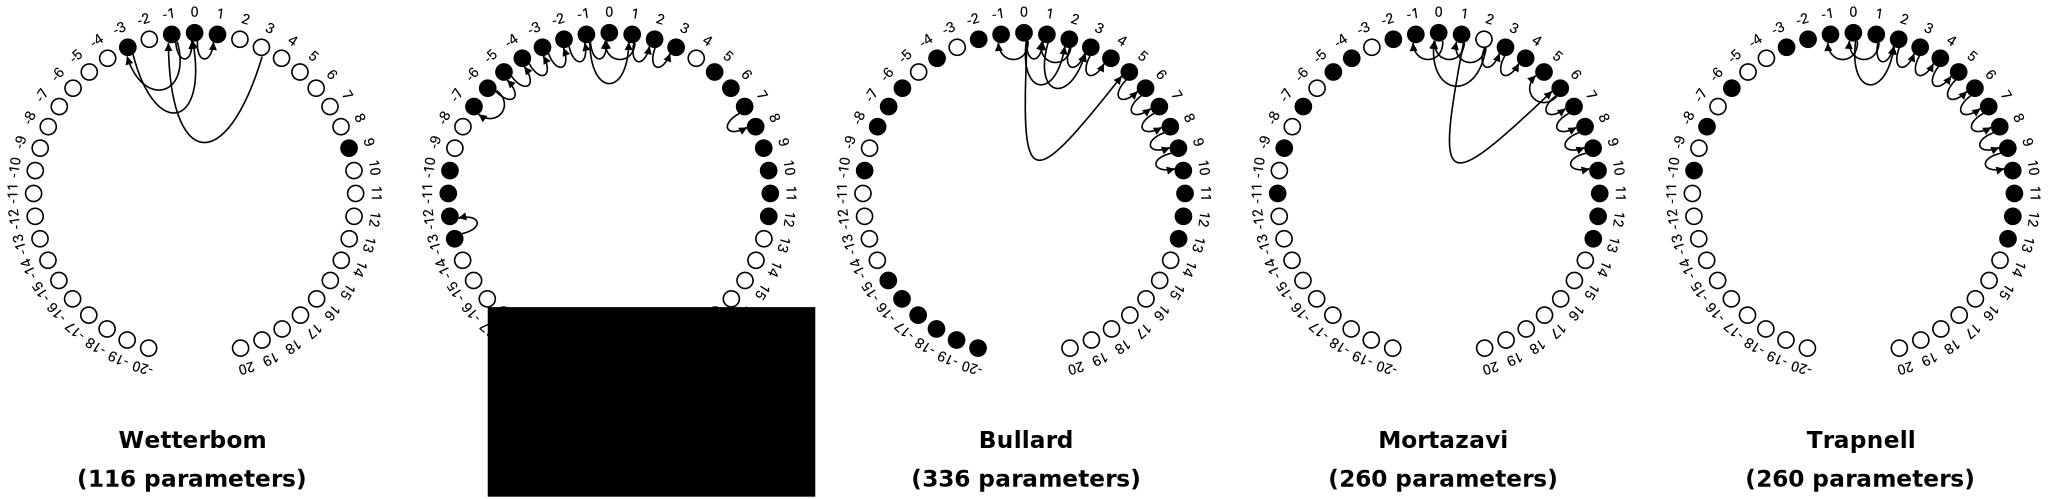
\includegraphics[width=\textwidth]{fig/models.eps}}
%% TODO: caption
\caption{Blah blah blah.}
\label{fig:models}
\end{figure*}


Because we cannot observe directly the underlying RNA-abundance, our evaluation
strategy relies on testing two assumptions we make of an ideal, unbiased experiment.
\begin{enumerate}
\item Positional nucleotide frequencies (as in Figure \ref{fig:freqs}), measured
from reads within exons, should not differ greatly from frequencies measured by
sampling uniformly within the same exons.
\item Read counts across a single exon should follow, approxmiately, a Poisson
process.
\end{enumerate}

We applied our procedure (labeled ``BN'') as well as those as well as those of
\citet{Li2010} (``GLM'' and ``MART'') and \citet{Hansen2010} (``7mer''), which
are implemented in the R packages \texttt{mseg} and \texttt{Genominator},
respectively. Thhe procedures were applied to four publically available data
sets \citep{Bullard2010, Mortazavi2008, Trapnell2010, Wetterbom2010}, as well as
an unpublished data sets of our own (Table \ref{tab:datasets}).

\begin{table}
\processtable{Datasets on which the methods are evaluated.\label{tab:datasets}}
{
\begin{tabular}{lllr}\toprule
Experiment & Species & Platform & Read Length \\\midrule
\citet{Wetterbom2010} & Chimpanzee & ABI & 33 \\
Katze (unpublished) & Macaque & ABI & 50 \\
\citet{Bullard2010} & Human & Illumina & 35 \\
\citet{Mortazavi2008} & Mouse & Illumina & 33 \\
\citet{Trapnell2010} & Mouse & Illumina & 75 \\\botrule
\end{tabular}
}{}
\end{table}


Testing was performed by cross-validation. Each method was trained on data taken
from chromosomes 1--8 of the genome from which the reads were mapped (including
chromosomes 2a and 2b of the Chimpanzee genome). For evaluation, we drew a set
of long, highly expressed exons from the remaining chromosomes. In particular, for
each reference sequence, beginning with the set of exons annotated by Ensembl
release 60 \cite{Hubbard2009}, we removed any exons with known alternate splice
sites, then chose the top 1000 exons by read count, restricting ourselves those
at least 100nt long.

The differences in the methods being tested necessitated training procedures
unique to each.

\citet{Li2010} recommends that their MART and GLM models be trained using the
100 most abundant genes. We used 1000 exons from chromosomes 1--8, otherwise
chosen in a manner identical to that which was used to select the test exons.
Both the GLM and MART models were trained using the default parameters.

\citet{Hansen2010} recommends using all of the reads to estimate heptamer
frequencies used by their model. The training procedure works by simple tallying
of frequencies. The implementation of this model in the Genominator package we
found to use a great deal of memory, and were unable to train with the volume of
data we wished, so we reimplemented the model and trained it on all of the reads
aligned to chromosomes 1-8.

We evaluated several variations of the heptamer model. The suggested method
involved averaging the frequencies of the first two heptamers of each read. Yet,
we found that in every case, this performed worse than simply counting the
frequencies of the initial heptamer, and thus we report only the latter. The
background frequences are estimated from positions 18--23 in each read.

Our own method was trained on the 200,000 reads from chromosomes 1--8, with the
highest number of duplicates.

All data sets were mapped using Bowtie \citep{Langmead2009} against the latest
genome assemblies available from the UCSC Genome Browser \citep{Karolchik2008}
during preparation.



\subsection{Kullback-Leibler Divergence}

Plotting the nucleotide frequencies (Figure  \ref{fig:freqs}) we observe an
obvious bias. To quantify the non-uniformity observed in these plots, we use the

If $f_x$ is the background frequency of a $k$-mer $x$, and $f'_x$ the observed
frequency, the KL divergence is computed as, symmetrized Kullback-Leibler (KL)
divergence \citep{Kullback1951}.
%Comparing only nucleotide frequencies may miss
%dinucleotide or higher order bias. Thus, for a fair comparison, we compute the
%KL divergence for $k$-mers, with $k \in \{ 1 \dots 6 \}$.
$$D_k( f, f' ) = \sum_{x} \left( f_x \log( f_x / f'_x ) + f'_x \log( f'_x / f_x) \right)$$
where the sum is over all $k$-mers.


%% --------------------

To avoid the risk of a small number of reads with many duplicates dominating the
measure, we do not count duplicate reads when computing the KL divergence. Since we
explicitly chose exons with high coverage, not counting duplicates may not
fully capturing the effects of the bias correction methods. Thus, for each exon,
we compute the number of duplicates for each read, and count only reads in the
upper half. Under the assumption of uniform sampling, the set of reads falling
in the upper half should not depend on sequence, and we should expect the KL
divergence to be low.

We compute the divergence by reweighting the read counts using the predicted
bias coefficient, choosing the upper half in each exon, discarding duplicate
reads, and then tallying frequencies of overlapping $k$-mers. The $k$-mer
distribution obtained are then compared to a background distribution obtained by
redistributing reads uniformly at random within their exons.

We repeated the procedure for $k \in \{1, 2, 3, 4, 5, 6\}$. The results of this
analysis are plotted in Figure \ref{fig:kl}, for $k = 1$ and $k = 4$. The
remaining cases are plotted in Supplementary Section 3.
%% TODO: what section, for real?

\begin{figure*}
\centerline{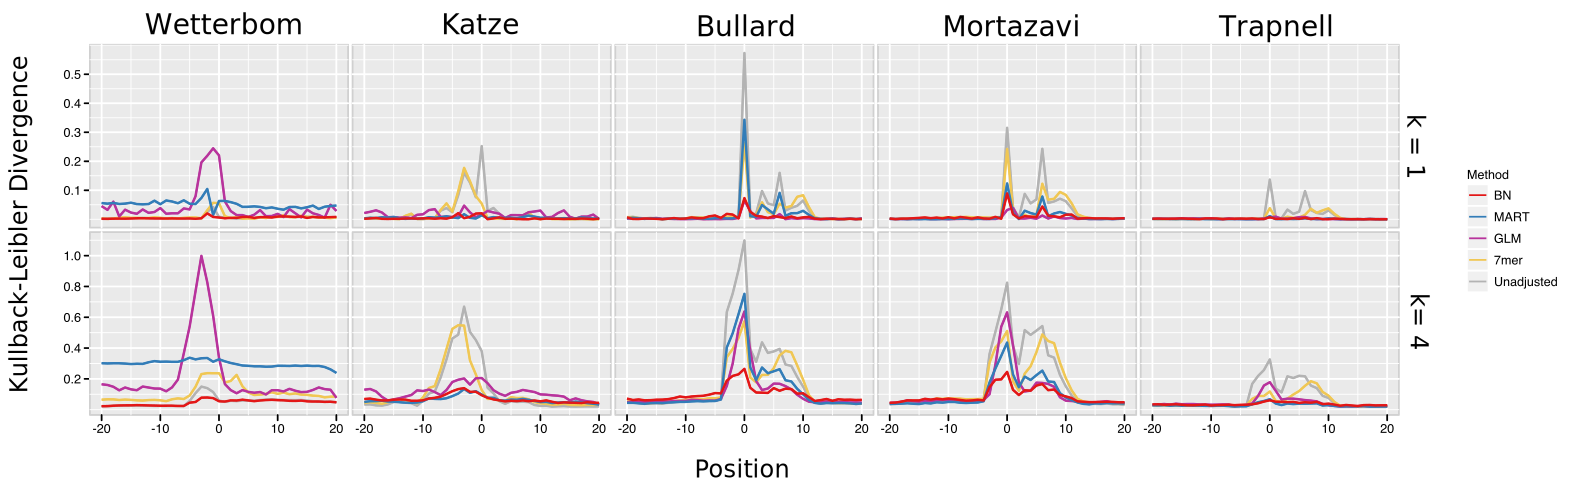
\includegraphics[width=0.9\textwidth]{fig/kl.eps}}
\caption{The Kullback-Leibler divergence compares the frequency of $k$-mers
(here, for $k = 1$ and $k = 4$) surrounding the starts of aligned reads to the
frquencies expected under the assumption of unifom sampling from within exons.
A large divergence indicates significant bias. Plotted here is the divergence
from unadjusted reads counts as well as after adjusting reads counts using each
method.}
\label{fig:kl}
\end{figure*}


\subsection{Poisson Regression}

In this comparison, we measure how well the counts conform to a Poisson process.
The assumption of positional read counts following a Poisson distribution is
known to be a poor fit \citep{Srivastava2010}, but measuring the improvement in
the fit derived from correcting for bias remains a principled and easily
interpreted criterion.

We perform maximum-likelihood fitting of two models. In the null model, the
Poisson rate is fixed for each exon. That is, for position $j$ within
exon $i$, the rate is
$$ \lambda_{ij} = a_i $$
where $a_i$ is the parameter being fit. For comparison, we then fit a model in
which the rate is also proportional to the predicted bias coefficients:
$$ \lambda'_{ij} = a_i b_{ij} $$

If the null model has log-likelihood $L$, and the bias-corrected model $L'$, a
simple goodness of fit measure is the improvement in log-likelihood (a statistic
commonly known as McFadden's pesudo-coefficient of determination
\citep{McFadden1974}), defined as,
$$R^2 = 1 - \frac{L'}{L}$$

This measure can be interpreted as the improvement in fit over the null model,
with $R^2 = 1$ indicating a prefect fit, and a negitve numbers, an increasingly
worse fit. A more dubious, yet intuitive interpretation of $R^2$ is the
proportion of variability eplained by the model.

We compue $R^2$ for each of the test exons, giving us a sense of the variability
of the effectiveness of each model. The results of this analysis are plotted in
Figure \ref{fig:pois}.  To summarize each model with a single number, we can
examine the median $R^2$ value, as listed in Table \ref{tab:pois}.

\begin{figure}
\centerline{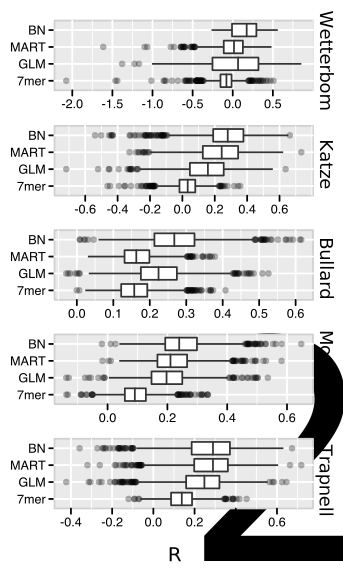
\includegraphics[width=0.3\textwidth]{fig/pois-boxplot.eps}}
\caption{For each of the 1000 test exons, we measure a pseudo-coefficients of
determination $R^2$, equivalent to the improvement in log-likelihood under the
bias corrected model. The statistic is positive when uniformity is increased,
and negative when decreased. Boxes are plotted to mark the 25\%, 50\%, and 75\%
quantiles, with whiskers extending to 1.5 times the inter-quartile range (i.e.,
the span between tho 25\% and 75\% quantiles).
}


    \label{fig:pois}
\end{figure}


\begin{table}
\processtable{
    The $R^2$ goodness of fit statistic measures increased uniformity in read
    coverage, after correcting for bias. Here the median $R^2$ across the test
    exons is listed for each method and simple. A positive $R^2$ indicates a
    better fit.\label{tab:pois}}{
    \begin{tabular}{lcccc}\toprule
          & BN    & MART  & GLM   & 7mer \\\midrule
Wetterbom & 0.173 & 0.016 & 0.066 & -0.079 \\
Katze     & 0.286 & 0.243 & 0.158 & 0.033 \\
Bullard   & 0.276 & 0.163 & 0.224 & 0.157 \\
Mortazavi & 0.248 & 0.210 & 0.197 & 0.091 \\
Trapnell  & 0.308 & 0.289 & 0.248 & 0.138
    \end{tabular}
}{}
\end{table}



\section{Discussion}

We have demonstrated that sequence bias can confound, sometimes severely,
quantification in RNA-Seq experiments, and we have introduced an effective
method to account for this bias without the need of existing gene annotations.

In our results, estimating initial heptamer frequencies was not seen to be as
effective as the other models, even when data generated using random hexamer
priming was used. Given the large number of parameters needed to estimate
heptamer frequencies, a likely explanation is that the model is overfit to the
training set. Though the training set consisted of at least 600,000 reads in
each experiment, it seems more reads, or a greater diversity of reads are needed
to produce an accurate or useful estimate.

Our method generalizes this approach, attempting to overcome this problem by
using an estimation of sequence probability that is more robust to overfitting
and can account for bias beyond the initial heptamer. In all our tests, this
approach was at least as effective as those of \citet{Li2010}, despite not
requiring gene annotations, or manual selection of training examples.

We have withheld any direct comparison to the method described by
\citet{Roberts2011} and implemented in Cufflinks \citep{Trapnell2010}. Though
this method is superficially similar to our own, a proper comparison is
difficult, as the software can not be applied independently of estimating
transcript abundance in FPKM using Cufflinks. Fairness would dictate that
competing methods be substituted in FPKM estimation, or that a seperate
interface be written to the Cufflinks bias correction method---both comparison
requiring significant effort.

Though the Cufflinks method and our own both use graphical models to estimate
sequence probabilities, we make no restriction on the graph other than
acyclicity, and go to considerable effort to efficiently approximate the optimal
structure for each data set, rathor than using a fixed structure, as in
Cufflinks. A ``one size fits all'' approach likely works quite well in many
cases, yet the observed specificity of the bias to protocal and platform argues
against it. For example, the structures learned by our method (Figure
\ref{fig:models}), are considerably different between those sequenced on an
Illumina platform versus an AB platform.

%% TODO: discussion of run-time, etc


Because we do not require annotations, CHiP-Seq, and other high-throughput
sequencing experiments may also benefit from our model. In a preliminary
investigation, we found the sequence bias in one CHiP-Seq experiment
\cite{Cao2010} was less than that observed in any of the RNA-Seq data we
evaluated, however our method is still able effectively correct for the bias
that was observed (see, Supplementary Section 4).
%% TODO: which actual section ?
Protocol differences, as we have seen,
can result in significant differences in observed nucleotide frequencies, so we
may not safely assert that bias in CHiP-Seq data is always low.  Given the weak
assumptions made by our model, our estimation of bias could easily be
incorporated into CHiP-Seq peak calling algorithms, and potentially improve
accuracy.

RNA-Seq is most often used to compare levels of expression, and so a natural
concern is the consistency of the bias between samples. In the data we examined,
the bias appears to be largely, but not entirely consistent (see,
Supplementary Section 5).
%% TODO: which actual section ?
Similarly, in Figure \ref{fig:freqs}, the three data sets
sequenced on the Illumina platform display similar patterns of nonuniformity,
yet differ in magnitude. Batch effects in RNA-Seq remain a legitimate concern,
that should be evaluated and corrected for.


\bibliographystyle{natbib}
\bibliography{seqbias-paper}

\end{document}



